\documentclass {article}
\usepackage{amsmath}
\setlength{\parindent}{0cm}

\usepackage{hyperref}
\usepackage{graphicx}
\usepackage{subcaption}
\usepackage[margin=1.5in]{geometry}

\usepackage{fancyhdr}
\pagestyle{fancy}
\lhead{\textbf{Complex Network Analysis} \\ Assignment 3\\}
\rhead{Maria Kagkeli \\ Maria Regina Lily \\ Mihai Verzan}
\headheight 10pc
\voffset -10pc

\begin{document}



% problem 1
\section{Clustering Coefficients}

\subsection{}

$ k_{A, B} = \ell + 1$, $k_{\ell} = 2 $, so:
\begin{align*}
\langle C \rangle & = \frac{ 1 }{ N } \sum\limits_{ i=1 }^N \frac{ 2 L_i }{ k_i (k_i - 1) } \\ \\
& = \frac{ 1 }{ N } \left( \underbrace{\sum\limits_{ A,B } \frac{ 2 \ell }{ (\ell + 1) \ell }}_\text{nodes $A$, $B$} + \underbrace{ \sum\limits_{ i=0 }^{N-2} \frac{ 2 \cdot 1 }{ 2 \cdot 1 }}_\text{nodes $l$} \right) \\ \\
& = \frac{ 1 }{ N } \left( \frac{ 4 }{ \ell + 1 } + N - 2  \right) \\ \\
& = \frac{ 1 }{ N } \left( \frac{ 4 }{ N - 1 } + N - 2  \right) \\ \\
& = \frac{ 1 }{ N } \left( \frac{ 4 + (N - 2)(N - 1) }{ N - 1 } \right) \\ \\
& = \frac{ 1 }{ N } \left( \frac{ 4 + N^2 - 3N + 2 }{ N - 1 }  \right) \\ \\
& = \frac{ N^2 - 3N + 6 }{ N^2 - N }. \\ \\
\end{align*}

\subsection{}

\text{According to hint:}
\begin{align*}
C_{\Delta} &= \frac{ 3 \cdot \# triangles }{ \# triples },
& \# triples = \sum\limits_{ i=1 }^N \frac{ k_i (k_i - 1) }{ 2 }.\\
\end{align*}

In the given graph, $ \# $ triangles = $ \ell $, therefore:
$$ C_{\Delta} = \frac{ 3 \ell }{ \sum\limits_{ i=1 }^N \frac{ k_i (k_i - 1) }{ 2 }}. $$
 
From problem 1.1: $ k_{A, B} = \ell + 1$,    $k_{\ell} = 2 $, so:
\begin{align*}
 C_{\Delta} &=   \frac{ 3 \ell }{ \sum\limits_{ A,B} \frac{ (\ell + 1) \ell }{ 2 } + \sum\limits_{ i=0 }^{N-2} \frac{ 2 \cdot 1 }{ 2 }} \\ \\
& =\frac{ 3 \ell }{ \ell (\ell + 1) + N - 2 } \\ \\
& = \frac{ 3 (N - 2) }{ (N-1)(N-2) + N - 2 } \\ \\
& = \frac{ 3 (N - 2) }{ N^2 - 3N + 2 + N - 2 } \\ \\
& = \frac{ 3 (N - 2) }{ N^2 - 2N } \\ \\
& = \frac{ 3 (N - 2) }{ N (N - 2) } \\ \\
& = \frac{ 3 }{ N }.
\end{align*}

\subsection{}
As $ N \to \infty $, the average clustering coefficient $ \langle C \rangle = (\frac{ N^2 - 3N + 6 }{ N^2 - N }) $ goes to $ 1 $. These reflects the fact that nodes $ A $ and $ B $ are connected to all others, and as the number of nodes goes to infinity, these connections dominate the coefficient. The global clustering coefficient $ C_{\Delta} = \frac{ 3 }{ N } $ goes to 0, meaning that the number of triangles grows much more slowly than the number of triples. These limits show that in some cases, there is a very clear difference between the two formulations. 

\newpage



% problem 2
\section{Watts-Strogatz Network Model}

\subsection{}

Minimum average clustering coefficient: when $ p = 0 $: $ \langle C(0) \rangle = \frac{ 3(2m-2) }{ 4(2m-1) } $. As m grows, $ \langle C(0) \rangle \to \frac{ 3 }{ 4 } $.

Maximum average clustering coefficient: when $ p = 1 $. The network becomes random: $ \langle C(1) \rangle = \frac{ 2m }{ N } $. 

\subsection{}

Minimum average shortest path: when $ p = 0 $: $ \langle d(0) \rangle = \frac{ N }{ 4m } $.

Maximum average shortest path: when $ p = 1 $: $ \langle d(1) \rangle = \frac{ \ln N }{ \ln 2m } $.

\subsection{}
Find $ N $ by counting the nodes: $ N = 12 $.

Find $ m $ by counting how many neighbouring nodes each node is connected to. While not all links will be present due to the random rewiring, a large portion of nodes are connected to the nodes right next to themselves, as well as the next nodes over, so $ m = 2 $ is a reasonable estimate.

Out of the 24 initial links, 21 are preserved and 3 have been rewired. Therefore we can estimate $ p \approx \frac{ 3 }{ 21 } = \frac{ 1 }{ 7 } $.

\newpage



% problem 3
\section{Kleinberg Network Model}

Note: plots and discussion also given in asg03-3.ipynb.

\subsection{}
-- implemented in asg03-3.ipynb --

\subsection{}
\begin{figure}[h!]
  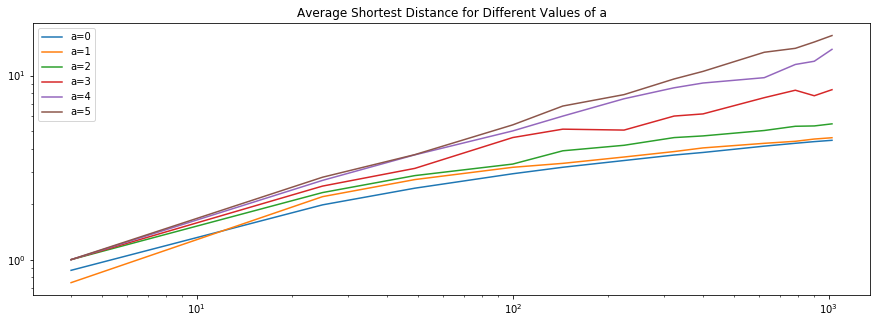
\includegraphics[width=\linewidth]{img/2.png}
\end{figure}

\subsection{}
For higher values of $ a $ ($ a=4 $, $ a=5 $), the average shortest distance $ <d(N)> $ grows approximately proportional to $ log(N) $. This means, the Kleinberg model generates networks with small-world-behaviour for higher values of $ a $

\subsection{}
\begin{figure}[h!]
  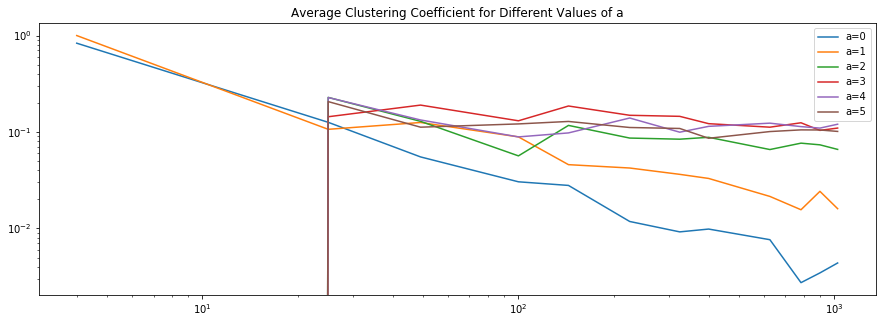
\includegraphics[width=\linewidth]{img/4.png}
\end{figure}

We can see here that the average clustering coefficient for the lower values of $ \alpha $, ($ \alpha = 0, 1, 2 $), the average clustering coefficient is inversely proportional to the $ log(N) $

For the higher values of $ \alpha $, ($ \alpha = 5, 4, 3 $), the average clustering coefficient increase significantly between $ N=10 $ and $ N=100 $. But generally, the average clustering coefficient stays rather low for higher values $ \alpha $.

This reflects the weighted random selection of the extra link that would be added to each node. The neighbors $ y $ of a node $ x $ would have the distance $ d(x,y)=1 $, which would give these neighbors the highest chances of being picked as target node of the extra link. As a result, the chances of the graph actually getting new links for high values of $ \alpha $ is rather small. If no new link is created, then the average clustering coefficient would be $ 0 $ , or near to $ 0 $. (As we found in the previous assignment, a grid-like lattice network has the average clustering coefficient of $ 0 $)

\end{document}